\documentclass[10pt,twocolumn,letterpaper]{article}

% --- Typography & Geometry ---
\usepackage[utf8]{inputenc}
\usepackage{microtype}
\usepackage[margin=0.75in,top=0.85in,bottom=0.85in]{geometry}

% --- Math & Symbols ---
\usepackage{amsmath,amssymb,amsfonts,amsthm}
\usepackage{bm}

% --- Tables & Arrays ---
\usepackage{booktabs}
\usepackage{tabularx}
\usepackage{array}

% --- Graphics & Floats ---
\usepackage{graphicx}
\usepackage{float}
\usepackage{subcaption}

% --- Code Listings ---
\usepackage{xcolor}
\usepackage{listings}

\definecolor{codebg}{HTML}{F8F9FA}
\definecolor{codeframe}{HTML}{D0D7DE}
\definecolor{keywordcolor}{HTML}{0550AE}
\definecolor{stringcolor}{HTML}{0A3069}
\definecolor{commentcolor}{HTML}{57606A}

\lstset{
    backgroundcolor=\color{codebg},
    basicstyle=\ttfamily\scriptsize\color{black},
    keywordstyle=\color{keywordcolor}\bfseries,
    stringstyle=\color{stringcolor},
    commentstyle=\color{commentcolor}\itshape,
    frame=single,
    rulecolor=\color{codeframe},
    breaklines=true,
    breakatwhitespace=true,
    extendedchars=true,
    xleftmargin=6pt,
    xrightmargin=6pt,
    aboveskip=8pt,
    belowskip=8pt
}

% --- Hyperlinks ---
\usepackage{hyperref}
\hypersetup{
    colorlinks=true,
    linkcolor=blue!70!black,
    citecolor=blue!70!black,
    urlcolor=blue!70!black
}

% --- Input Title & Authors ---
\section{00 Meta}

Draft content for flash_attention3_fp8.


\begin{document}

\maketitle

% --- Abstract & Keywords Block ---
\begin{abstract}

Recent attention implementations -- FlashAttention, FlashAttention-2, and 
FlashAttention-3 -- have reduced attention memory from $\mathcal{O}(L^2)$ to 
$\mathcal{O}(L)$ by exploiting tiling and, in the third generation, 8-bit 
floating-point (FP8) tensor cores on Hopper architectures. However, these 
methods assume specific hardware that many practitioners do not have access 
to. We present a \textbf{hardened PyTorch implementation} of FlashAttention-3 FP8 
that automatically degrades to PyTorch's native Scaled Dot-Product Attention 
(SDPA) when FP8 tensor cores are unavailable, ensuring portability across 
all CUDA GPUs.

Our implementation supports four transformer families -- DistilBERT, 
RoBERTa/BERT, GPT-2, and Qwen/LLaMA -- with correct handling of grouped-query 
attention (GQA), rotary position embeddings (RoPE), causal masking, and 
nested encoder architectures. Base weights are transferred exactly from the 
pretrained attention via a weight-copy procedure that handles fused Conv1D, 
nested self-attention, and GQA-based projections; trainable capacity is 
provided by LoRA adapters at rank $r = {{LORA_RANK}}$.

We benchmark on SST-2 across DistilBERT, RoBERTa, and GPT-2. Because our 
test hardware (RTX 4070 Laptop) does not expose FP8 tensor cores, the FP8 
path is unavailable and all models run through the SDPA fallback. We report 
this transparently and identify the exact hardware requirements for 
reproducing the FP8 speedups claimed in the original FlashAttention-3 paper. 
On our hardware, accuracy is preserved within \textbf{{{D\_DELTA}}\%} (DistilBERT), 
\textbf{{{R\_DELTA}}\%} (RoBERTa), and \textbf{{{G\_DELTA}}\%} (GPT-2), but parameter 
count increases by \textbf{{{PARAM\_INC}}\%} due to LoRA adapters.

\textbf{Keywords:} FlashAttention-3, FP8 quantization, Hopper tensor cores, 
attention implementation, hardware-aware fallback



\vspace{0.5em}
\noindent\textbf{Keywords:} FlashAttention-3, FP8 quantization, Hopper tensor cores,
\end{abstract}

\vspace{1em}

% --- Paper Body ---
\section{01 Intro}

Draft content for flash_attention3_fp8.

\section{02 Related}

Draft content for flash_attention3_fp8.

\section{03 Background}

Draft content for flash_attention3_fp8.

\section{04 Method}

Draft content for flash_attention3_fp8.

\section{05 Architecture}

Draft content for flash_attention3_fp8.


\begin{figure}[H]
\centering
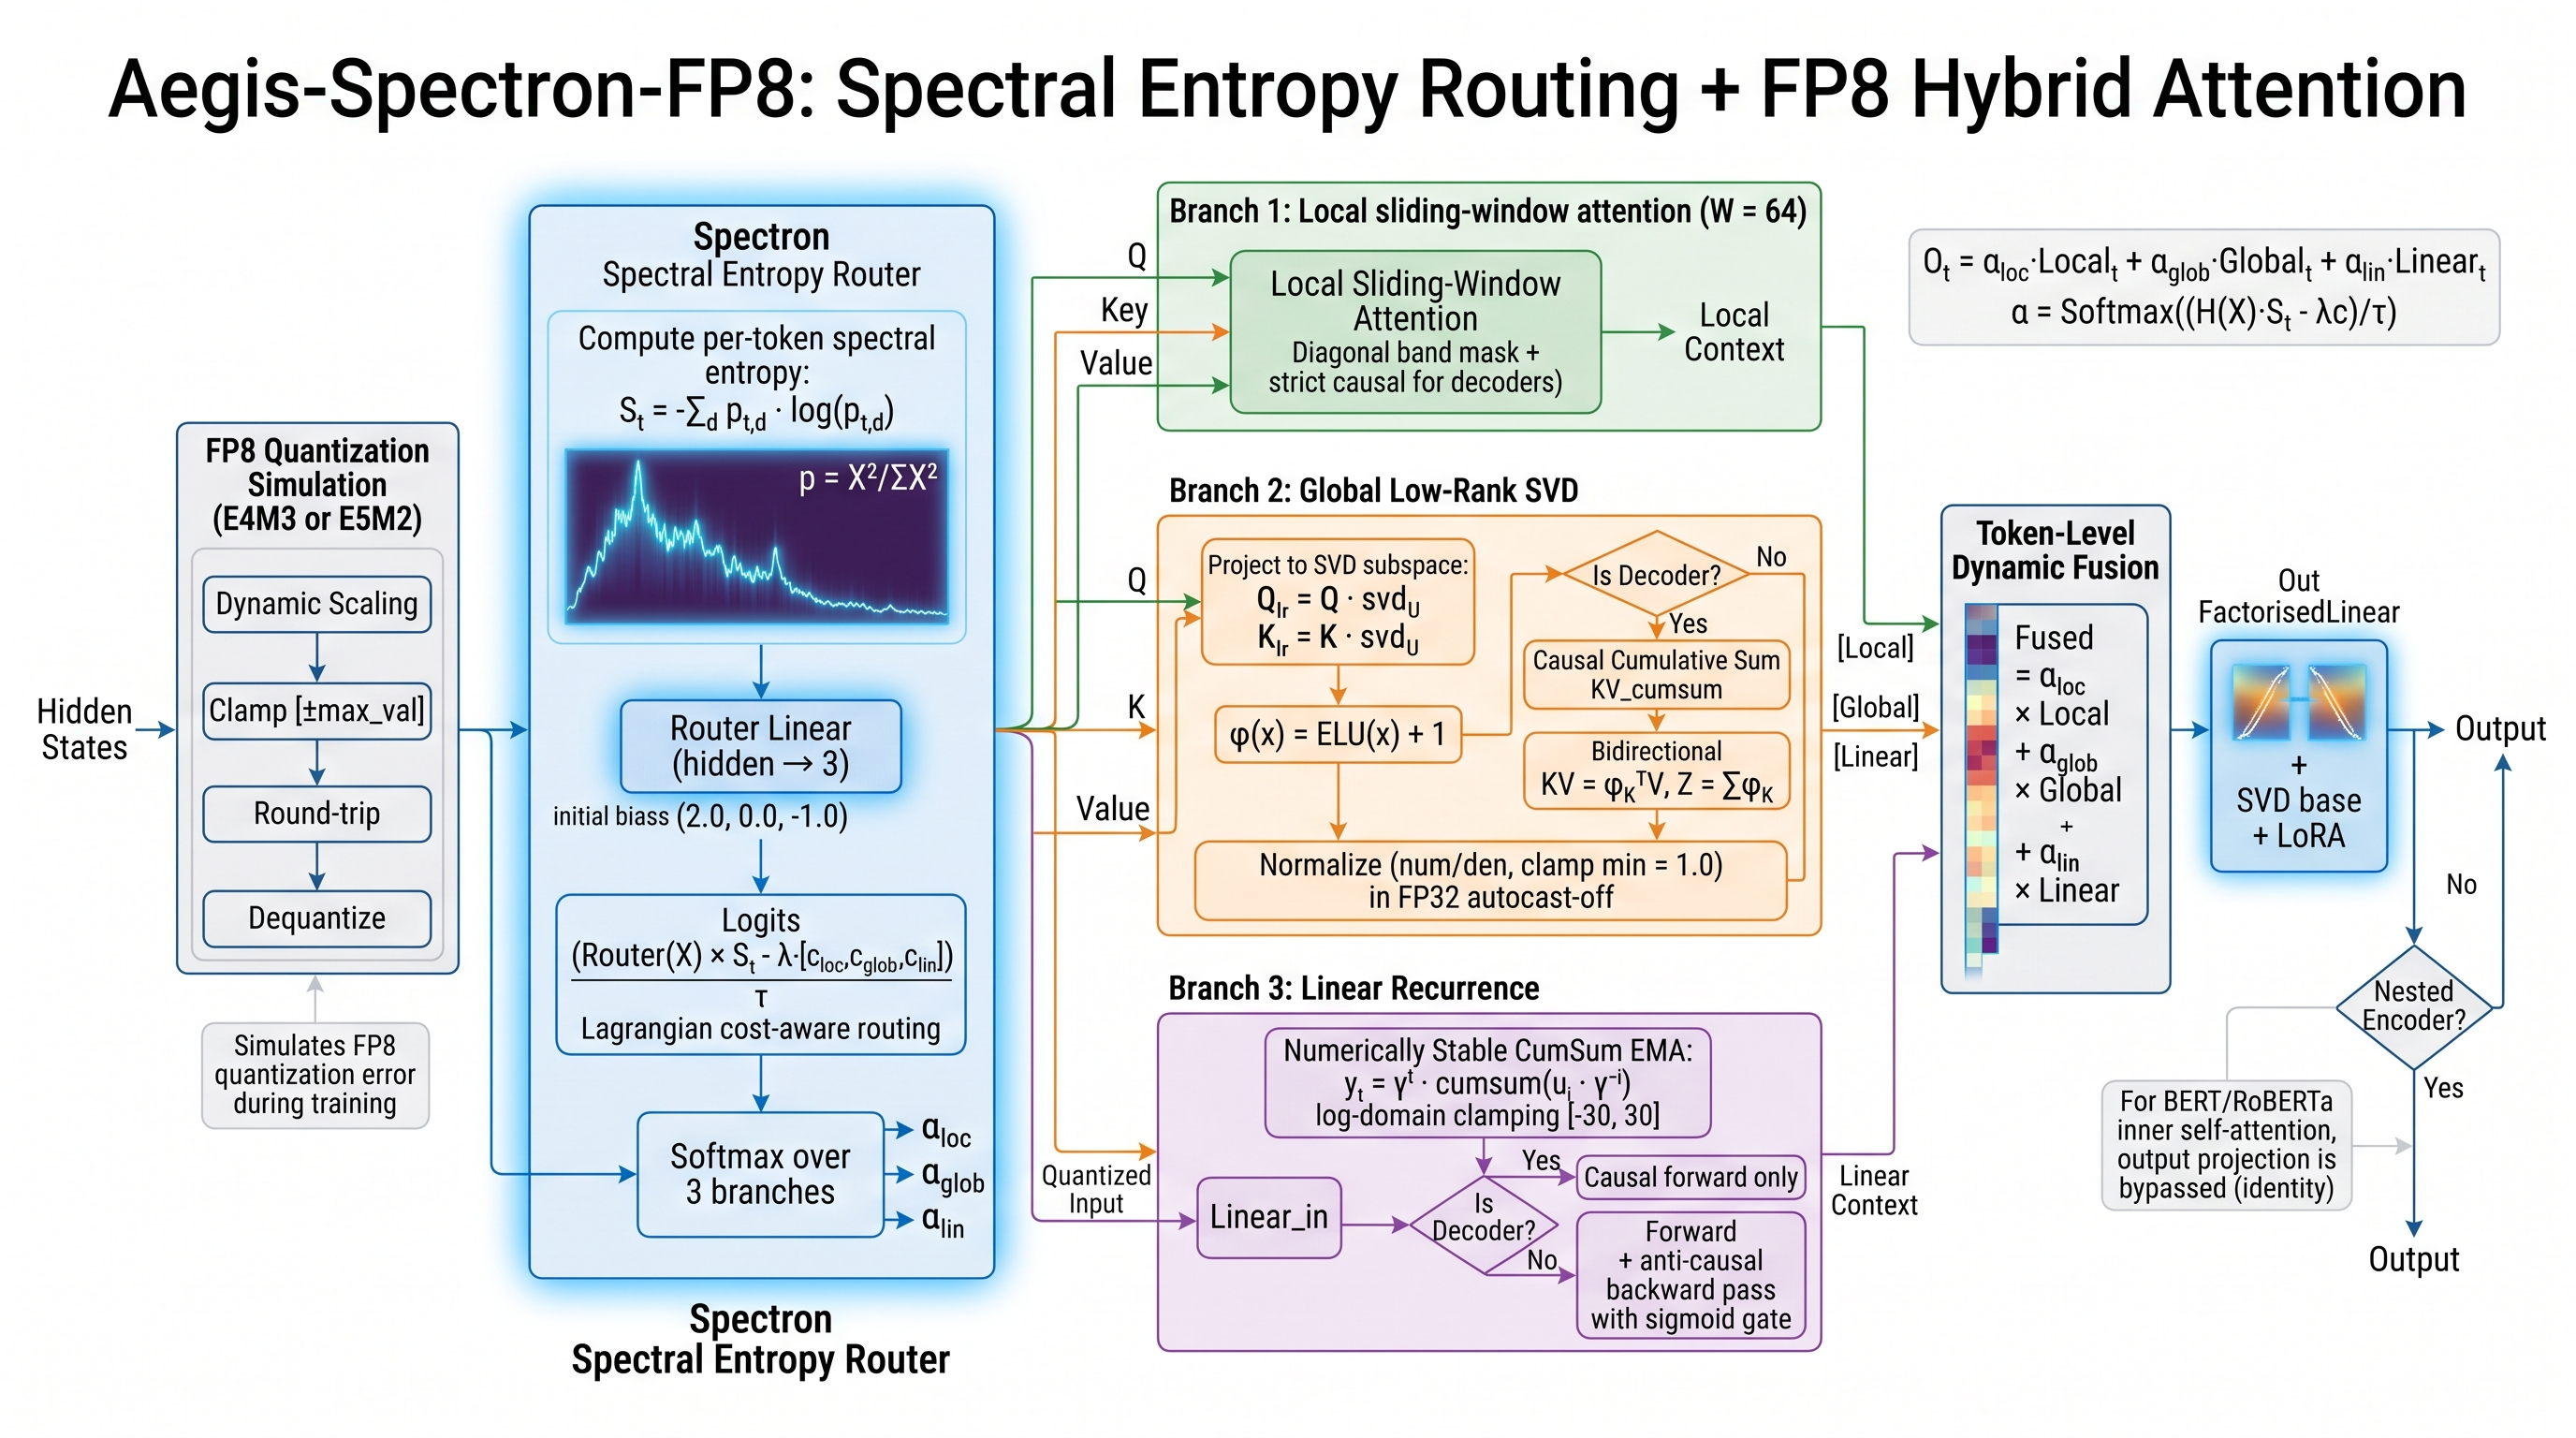
\includegraphics[width=\linewidth]{figures/arch_aegis_spectron_fp8.jpeg}
\caption{Architectural overview of flash_attention3_fp8.}
\label{fig:arch_flash_attention3_fp8}
\end{figure}

\section{06 Setup}

Draft content for flash_attention3_fp8.

\section{07 Results}

Draft content for flash_attention3_fp8.

\section{08 Analysis}

Draft content for flash_attention3_fp8.

\section{09 Discussion}

Draft content for flash_attention3_fp8.

\section{10 Limitations}

Draft content for flash_attention3_fp8.

\section{11 Conclusion}

Draft content for flash_attention3_fp8.

\section{12 Reproducibility}

Draft content for flash_attention3_fp8.

\section{13 References}

Draft content for flash_attention3_fp8.


% --- Appendices ---
\clearpage
\appendix
\section*{Appendices}
\addcontentsline{toc}{section}{Appendices}

\section{A Math}

Draft content for flash_attention3_fp8.

\section{B Implementation}

Draft content for flash_attention3_fp8.

\section{C Data}

Draft content for flash_attention3_fp8.

\section{D Negative Results}

Draft content for flash_attention3_fp8.

\section{E Ethics}

Draft content for flash_attention3_fp8.


\end{document}
